\section{Features}

The x86 architecture employs several general-purpose registers, including EAX, EBX, ECX, EDX, ESI, EDI (utilized as source and destination indices for string operations), EBP (serving as the base pointer), and ESP (acting as the stack pointer). 
Additionally, it incorporates:
\begin{itemize}
    \item The instruction pointer (EIP) in x86 architecture remains inaccessible directly, but undergoes modification through instructions like \texttt{jmp}, \texttt{call}, and \texttt{ret}. 
        Its value can be retrieved from the stack, known as the saved IP. 
        This register is 32 bits in size and serves as a holder for boolean flags that convey program status, including overflow, sign, zero, auxiliary carry (BCD), parity, and carry. 
        These flags indicate the outcome of arithmetic instructions and play a crucial role in controlling program flow.
        In terms of program control, the direction flag manages string instructions, dictating whether they auto-increment or auto-decrement. 
        Additionally, EIP controls system operations pertinent to the operating system.
    \item Program status and control are managed by the EFLAGS register.
    \item Segment registers are also utilized in the architecture.
\end{itemize}
The core data types include:
\begin{itemize}
    \item \textit{Byte}: 8 bits
    \item \textit{Word}: 2 bytes
    \item \textit{Dword} (Doubleword): 4 bytes (32 bits)
    \item \textit{Qword} (Quadword): 8 bytes (64 bits)
\end{itemize}

Assembly language is unique to each Instruction Set Architecture (ISA) and directly corresponds to binary machine code. 
The process of converting assembly language instructions into machine code is illustrated in the diagram below:
\begin{figure}[H]
    \centering
    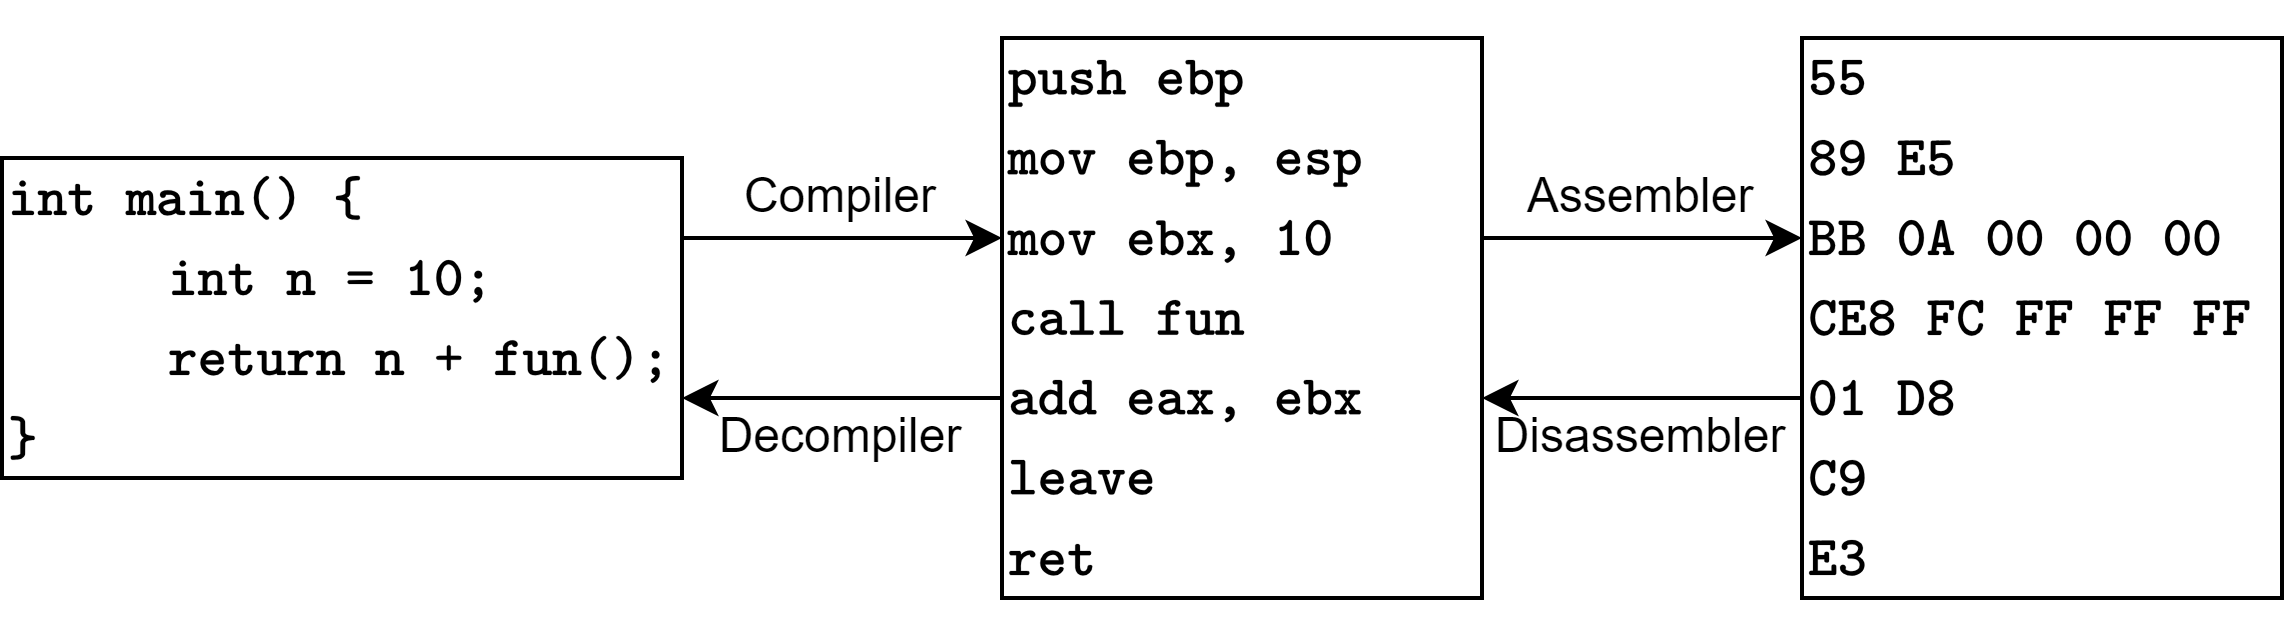
\includegraphics[width=0.75\linewidth]{images/assembler.png}
    \caption{From source code to machine code}
\end{figure}